\section{Avanserte pakkar}

\begin{frame}{Avanserte pakkar}

  Det vil ofte vera behov for ulike grafar og figurar i eit dokument. Dersom ein graf vert generert i eit eksternt program, og ein berre importerer eit \textit{bilde} av grafen i dokumentet vil det vera ei utfordring å sørga for at det er riktig skriftstørrelse, og skrifttype på teksten som er inne i grafen. Det er også tungvindt å gjera endringar i grafen sidan ein må (1 )inn i eit anna verktøy, (2) gjera endringane, (3) eksportera ei ny utgåve av \textit{bildet} før ein går tilbake til å jobba med dokumentet.

I \LaTeX{} løyser ein dette med ``Pgfplots'' pakken. Dette er ein pakke som kan plotta eksterne datasett (til dømes ein CSV-fil frå ei simulering eller måling), og matematiske uttrykk, som \(3x^2\).
  
  Det finnes også ei rekkje spesialiserte pakkar til \LaTeX tilpassa ulike fagområde, til dømes ``circuitikz'' for teikning av kretsskjema.
\end{frame}

\begin{frame}{Pgfplots}

  \begin{tikzpicture}
    \begin{axis}
      \addplot[color=blue,domain=0:0.04,samples=50]{sin(deg(2*3.14*50*x))};
    \end{axis}
  \end{tikzpicture}
  
\end{frame}

\begin{frame}{Pgfplots}

  \begin{tikzpicture}
\begin{axis}
\addplot[color=red]{exp(x)};
\end{axis}
\end{tikzpicture}
%Here ends the 2D plot
\hskip 5pt
%Here begins the 3D plot
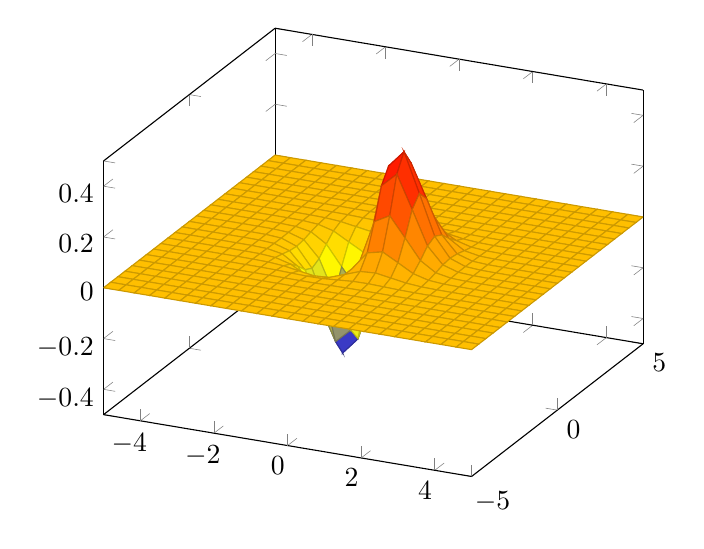
\begin{tikzpicture}
\begin{axis}
\addplot3[
    surf,
]
{exp(-x^2-y^2)*x};
\end{axis}
\end{tikzpicture}
  
\end{frame}


\begin{frame}{circuitikz}


  
\end{frame}

%%% Local Variables:
%%% mode: latex
%%% TeX-master: "../latex-presentation"
%%% End:
